\chapter{Vývojová dokumentácia}
\label{chap:vyvoj_dok}

Táto kapitola je zameraná pre programátorov, ktorých by bližšie zaujímali implementačné detaily a štruktúra nášho programu. Najprv si opíšeme ako skompilovať priložené zdrojové súbory práce a neskôr sa pozrieme na stavbu programu.

\section{Kompilácia}
V prílohe tejto práce sa nachádzajú zdrojové kódy nášho programu. Na ich úspešné skompilovanie budeme ale potrebovať splniť niekoľko požiadaviek:
\begin{itemize}
\item Podporovaná platforma na kompiláciu je momentálne iba Windows 10 verzie 20H2.
\item Ku kompilácii je potrebné Visual Studio 2019 verzie 16.9.0, a Windows 10 SDK verzie 10.0.19041.0
\item Qt verzie 5.15.0 \footnote{V dobe dokončovania práce bola najnovšia verzia Qt 6.1, ktorá by mala byť spätne kompatibilná, ale netestovali sme to.}
\end{itemize}

\subsection{Inštalácia Qt}

Keďže ku kompilácii budeme potrebovať samotné Qt, ukážeme si jeho inštaláciu v nasledujúcich krokoch (v prípade, že náš počítač už obsahuje požadovanú verziu Qt, môžeme tieto kroky preskočiť a prejsť na integráciu VS s Qt~\ref{kap4:sec:VS2019_qt}). Tu je nutné spomenúť, že sa jedná o online inštaláciu a budeme potrebovať pripojenie k internetu:
\begin{itemize}
\item Po kliknutí na odkaz https://www.qt.io/download sa nám otvorí internetový prehliadač so stránkou na stiahnutie Qt, kde vyhľadáme možnosť \uv{Downloads for open source users} a klikneme na \uv{Go open source}.

\item Na aktuálnej stránke nascrollujeme úplne dole, kde klikneme na zelené tlačidlo s nápisom \uv{Download the Qt Online Installer}.

\item Na aktuálnej stránke klikneme na \uv{Download}, čím sa nám stiahne \uv{Qt Online Installer}. Ten následne spustíme.

\item Ako prvé nás privíta obrazovka, ktorá od nás vyžaduje prihlásenie sa do nášho Qt účtu. Toto je bohužiaľ nutnosť a nie je možné bez toho pokračovať. V prípade, že nemáme žiadny vytvorený Qt účet, môžeme si ho vytvoriť priamo počas inštalácie a celé to nezaberie viac ako dve minúty. Potom klikneme na tlačidlo \uv{Next}.

 \item Teraz sa postupne preklikáme až po časť, kde máme možnosť si vybrať či chceme zasielať štatistické údaje počas používania Qt Creatoru. Tu si môžeme zvoliť ktorúkoľvek z možností podľa osobných preferencií a pokračovať ďalej v inštalácii.
 
\item Postupne sa dostaneme na obrazovku kde si zvolíme konkrétne komponenty, ktoré sa nám nainštalujú. Komponenty, ktoré sú zaškrtnuté necháme tak a rozklikneme možnosť Qt$\leftarrow$Qt 5.15.0 a zaškrtneme možnosť \uv{MSVC 2019 64-bit} a klikneme na \uv{Next} (obrázok~\ref{obr:kap4:inst_sel}).

\begin{figure}[!htb]
	\centering
	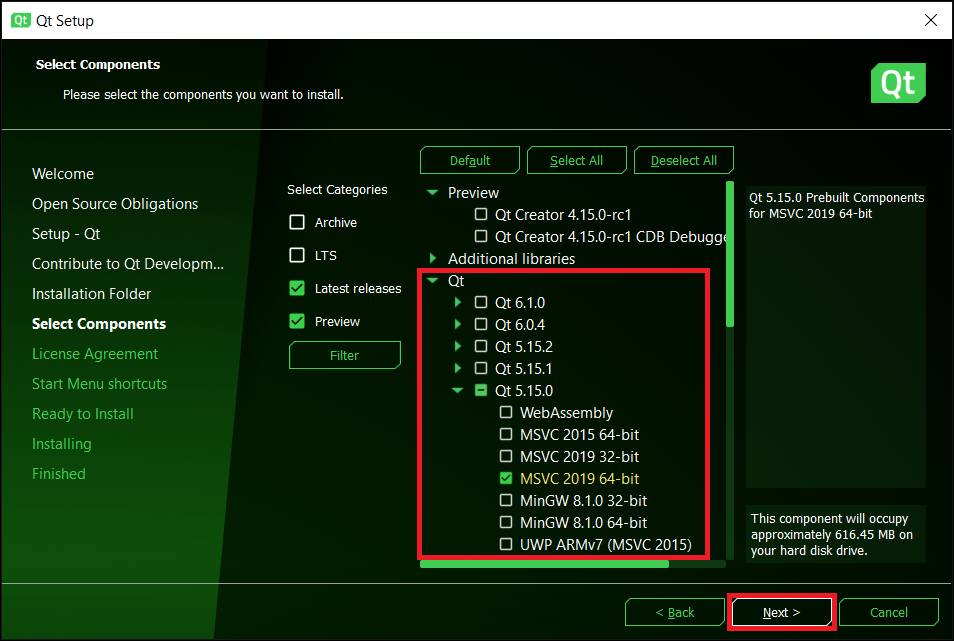
\includegraphics[width=12cm]{img/kap04_inst_sel}
	\caption{\uv{Select Components} časť Qt Setupu}
	\label{obr:kap4:inst_sel}
\end{figure}

\item Ďalej nasledujú bežné kroky pomocou ktorých dokončíme inštaláciu.

\end{itemize}

\subsection{Visual Studio 2019 a Qt}
\label{kap4:sec:VS2019_qt}
Teraz si ešte ukážeme integrovanie Visual studia 2019 spolu s Qt. Budeme si potrebovať nainštalovať \textit{Qt VS Tools}. Podrobný postup si ukážeme v nasledujúcich krokoch:
\begin{itemize}
\label{kap4:qt_vs_integ}
\item Priamo vo Visual Studiu si cez možnosť \textit{Extensions}$\rightarrow$\textit{Manage Extensions} do online hľadania zadáme \uv{Qt} a stiahneme si rozšírenie \uv{Qt Visual Studio Tools}~\cite{qt_vs_tools}
\item\label{kap4:qt_vs_integ:krok2} Po úspešnej inštalácii si musíme ešte vybrať Qt verziu cez možnosť \textit{Extensions}$\rightarrow$\textit{Qt VS Tools}$\rightarrow$\textit{Qt Versions} (ukázané na obrázku~\ref{obr:kap4:vs_versions}).

\begin{figure}[!htb]
	\centering
	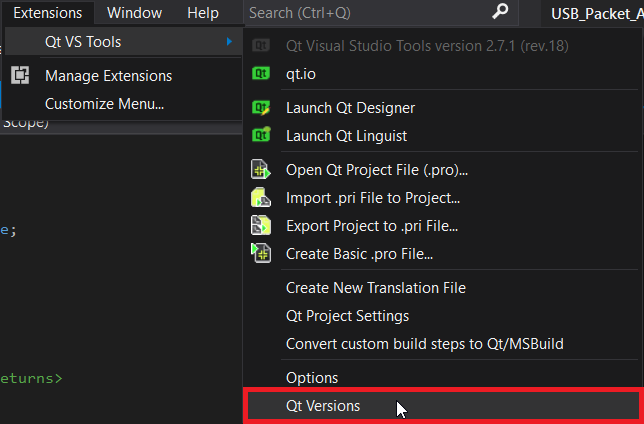
\includegraphics[width=12cm]{img/kap04_vs_versions}
	\caption{Visual Studio možnosť vybratia Qt verzie.}
	\label{obr:kap4:vs_versions}
\end{figure}

\item V dialógu sa teraz cez ikonu v stĺpčeku \uv{Path} (obrázok~\ref{obr:kap4:vs_path}) odkážeme do adresáru, kde sme nainštalovali \textit{Qt} a následne do adresáru \newline\textit{5.15.0\/msvc2019\_64\/bin} kde máme nainštalovaný \textit{qmake.exe}.

\begin{figure}[!htb]
	\centering
	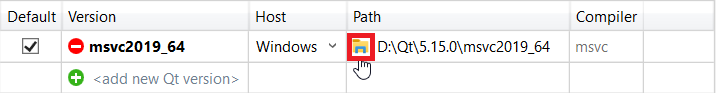
\includegraphics[width=12cm]{img/kap04_vs_path}
	\caption{Visual Studio zvolenie adresára ku \textit{qmake.exe}.}
	\label{obr:kap4:vs_path}
\end{figure}

\item Ako posledné si ešte skontrolujeme cez možnosť \textit{Project}$\rightarrow$\textit{Properties} v \textit{Configuration Properties}$\rightarrow$\textit{General} skontrolujeme, že máme nastavený \textit{C++ Language Standard} na možnosť \textit{ISO C++ 17} a \textit{Windows SDK Version} na verziu \textit{10.0.19041.0} ako na obrázku~\ref{obr:kap4:vs_prop}.

\begin{figure}[!htb]
	\centering
	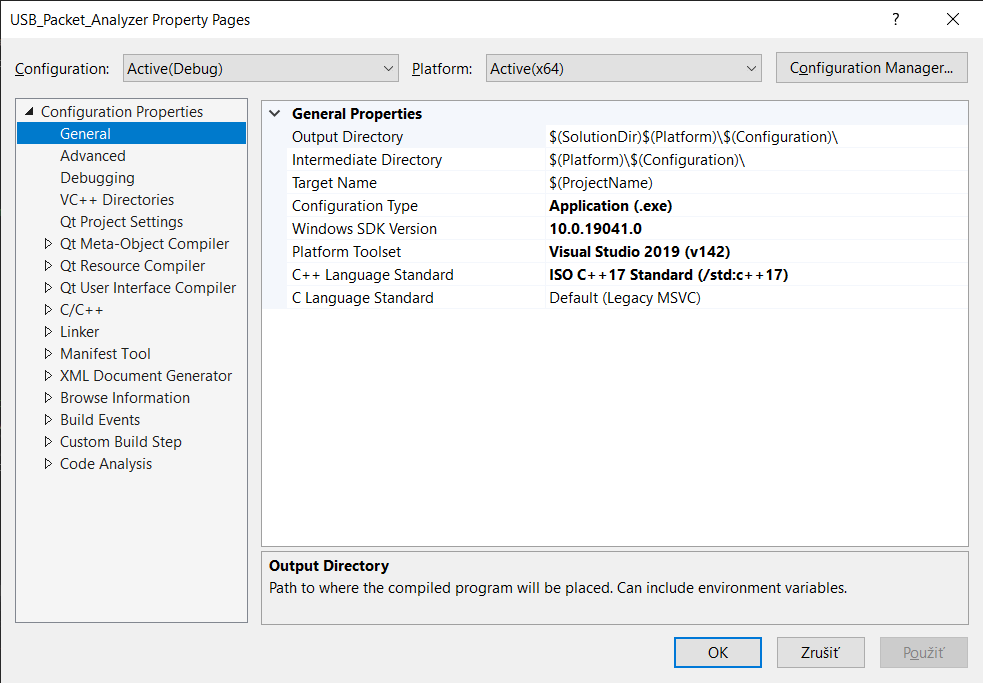
\includegraphics[width=12cm]{img/kap04_vs_prop}
	\caption{Visual Studio obecné nastavenia projektu.}
	\label{obr:kap4:vs_prop}
\end{figure}

\end{itemize}

\newpage
Môže sa stať, že narazíme na bug keď nám krok~\ref{kap4:qt_vs_integ:krok2} nenastaví Qt verziu a nebudeme vedieť projekt preložiť kvôli errorom typu \uv{cannot open source file qbytearray}. V takom prípade prejdeme do možnosti \textit{Project}$\rightarrow$\textit{Properties}$\rightarrow$\newline\textit{Qt~Project~Settings} a manuálne nastavíme \textit{Qt Installation} na \textit{msvc2019\_64} (obrázok~\ref{obr:kap4:vs_manual}).

\begin{figure}[!htb]
	\centering
	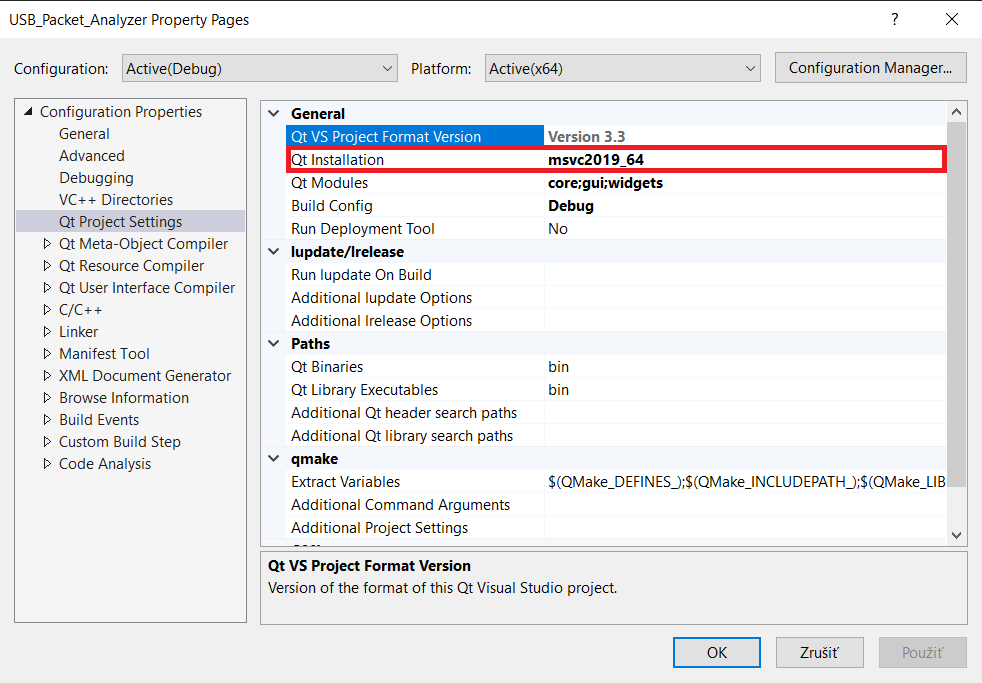
\includegraphics[width=12cm]{img/kap04_vs_manual}
	\caption{Visual Studio manuálne nastavenie Qt Installation.}
	\label{obr:kap4:vs_manual}
\end{figure}

V tomto momente by sme mali byť schopní úspešne skompilovať a spustiť náš program.

\subsection{Warningy pri kompilácii}
Warningy prekladaču sú samozrejme veľmi dôležité a nemali by byť ignorované. Niekedy sa ale jedná o vedľajší efekt, ktorý upozorňuje na časti kódu o ktorých sme si vedomí a neželáme si ich meniť. Pri kompilácii prázdneho Qt programu nám prekladač vygeneruje niečo cez 250 warningov a preto sme sa rozhodli niektoré z nich vypnúť v nastaveniach projektu. V časti \textit{Project}$\rightarrow$\textit{Properties}$\rightarrow$\newline\textit{Configuration Properties}$\rightarrow$\textit{C/C++}$\rightarrow$\textit{Advanced} sme do položky \textit{Disable Specific Warnings} pridali čísla nasledujúcich warningov, čím vypneme ich zobrazovanie:

\paragraph{C26812}~\cite{warningc26812} -- \uv{The enum type type-name is unscoped. Prefer 'enum class' over 'enum' (Enum.3)} -- tento typ warningu poukazuje aj na časti v našom kóde pretože používame tzv. \uv{plain enum} a porovnávame ho s položkami typu \texttt{int}, na ktoré majú plain enumy implicitnú konverziu.

Všetky nasledujúce warningy sa nachádzajú len v zdrojových kódoch Qt:
\paragraph{C26451}~\cite{warningc26451} -- \uv{Arithmetic overflow: Using operator 'operator' on a size-a byte value and then casting the result to a size-b byte value. Cast the value to the wider type before calling operator 'operator' to avoid overflow.}
\paragraph{C26498}~\cite{warningc26498} -- \uv{Use constexpr for values that can be computed at compile time.}
\paragraph{C26495}~\cite{warningc26495} -- \uv{Variable '\%variable\%' is uninitialized. Always initialize a member variable (type.6).}
\paragraph{C6011}~\cite{warningc6011} -- \uv{Dereferencing NULL pointer \textless~name\textgreater.}

\section{Architektúra aplikácie}

\begin{figure}[!htb]
	\centering
	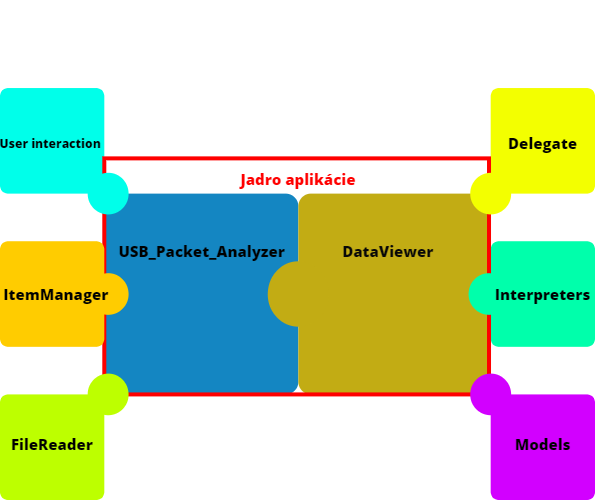
\includegraphics[width=\textwidth]{img/kap04_architektura}
	\caption{Diagram architektúry aplikácie}
	\label{obr:kap4:architek}
\end{figure}

V tejto sekcii si prejdeme celkovú stavbu aplikácie a akým spôsobom sú jednotlivé komponenty prepojené. Ako vidíme na obrázku~\ref{obr:kap4:architek}, aplikáciu môžeme rozdeliť do dvoch hlavných komponent, ktoré tvoria logické jadro programu: \texttt{USB\_Packet\_Analyzer} a \texttt{DataViewer}, na ktoré sa viažu ďalšie komponenty a dopĺňajú ich funkcionalitu. Teraz si podrobnejšie opíšeme obe hlavné komponenty spolu s komponentami, ktoré sú na nich napojené.

\section{USB\_Packet\_Analyzer}

USB\_Packet\_Analyzer tvorí hlavnú triedu programu, ktorá reprezentuje ok\-no zobrazené užívateľovi hneď po zapnutí aplikácie. Naše hlavné okno pozostáva z nasledujúcich komponent:
\begin{itemize}
\item QTableWidget -- slúži na vyobrazenie základných informácií o paketoch.
\item 2 QRadioButtony -- slúžia na výber medzi analýzou fixného súboru (file capture), alebo súboru do ktorého môže sniffer počas analýzy niečo pripísať (live capture).
\item QCheckBox -- slúži na výber, či užívateľ chce farebne zvýrazniť detailnejší význam analyzovaných paketov alebo nie.
\item QLabel -- slúži na vyobrazenie názvu súboru, ktorý sa aktuálne spracováva.
\item QProgressBar -- progress bar ukazujúci stav spracovania súboru počas file capture.
\item 5 QPushButtonov -- tlačidlá, ktorých jednotlivú funkcionalitu si vysvetlíme nižšie v tejto sekcii~\ref{kap04:sec:open_button}.
\end{itemize}
Zároveň implementuje funkcie spojené s užívateľskou interakciou, od ktorej sa následne odvíja ďalšie správanie aplikácie.

\subsection{Užívateľská interakcia}
Ako sme už spomínali vyššie v kapitole~\ref{kap3:sec:model_view}, Qt využíva na komunikáciu medzi objektami tzv. \uv{Signals \& Slots}~\cite{signal_slot} mechanizmus, ktorý funguje ako alternatíva ku callback funkciám v iných frameworkoch. Qt widgety majú veľa preddefinovaných signálov (ku ktorým si môžeme dodefinovať ďalšie), ktoré sú emitované pri konkrétnom evente (napríklad QPushButton~\cite{qpushbutton} má signál \texttt{clicked()} ktorý je emitnutý pokiaľ je dané tlačidlo stlačené). Slot je funkcia, ktorá je zavolaná ako odpoveď na konkrétny signál. Prepojenie signálu so slotom prebieha pomocou metódy \texttt{QObject::connect(QObject* sender, signal, QObject* receiver, method)}, kde postupne definujeme inštanciu QObject spolu s jej konkrétnym signálom a následne inštanciu QObject spolu s jej metódou, ktorá sa má zavolať po emitovaní daného singálu. Qt má takisto možnosť \uv{Auto-Connect}~\cite{qt_autoconnect} pri ktorej stačí, že sa budeme držať štandardných konvencií a tým pádom nebudeme musieť manuálne prepájať jednotlivé signály a sloty pomocou \texttt{connect()} metódy. Toto využívame napríklad pri tlačidlách, konkrétne so signálom \texttt{clicked()}, kde stačí ak si vytvoríme slot pomocou nasledujúcej mennej konvencie: \texttt{void on\_\textless object name \textgreater\_clicked()}.

\begin{figure}[!htb]
	\centering
	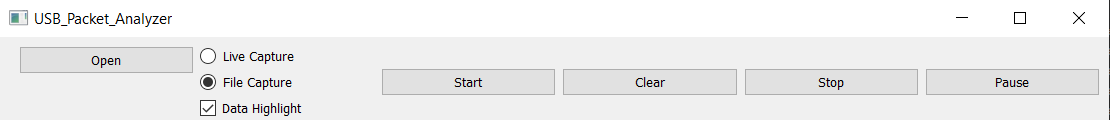
\includegraphics[width=\textwidth]{img/kap04_arch_buttons}
	\caption{Tlačidlá v aplikácii.}
	\label{obr:kap4:arch:buttons}
\end{figure}

Ako môžeme vidieť na obrázku~\ref{obr:kap4:arch:buttons}, naša aplikácia obsahuje hneď niekoľko tlačidieľ s odlišnou funkcionalitou o ktorú sa starajú už jednotlivé sloty, ktoré si teraz postupne opíšeme.

\paragraph{Open tlačidlo}
\label{kap04:sec:open_button}

slúži na vybratie si súboru na analýzu. To funguje na základe triedy QFileDialog~\cite{qfiledialog}, ktorá slúži na prechádzanie file systému. Užívateľovi sa zobrazí nový dialóg s intuitívnym ovládaním na ktoré je bežný užívateľ zvyknutý. Zároveň slúži na resetovanie progress baru a nastavenie labelu, ktorý zobrazuje aktuálne zvolený súbor.

\paragraph{Start tlačidlo}
\label{kap04:sec:start_button}

ako už napovedá jeho samotný názov, slúži na začatie analýzy. V tejto chvíli sa začne spracovávať súbor, ktorý si užívateľ zvolil pomocou predcházajúceho tlačidla Open~\ref{kap04:sec:open_button}. Spracovanie je následne vyobrazené pomocou QTableWidgetu, ktorým ako sme už riešili v kapitole~\ref{kap03:sec:zobr_zakl} vyobrazujeme základné informácie o jednotlivých paketoch. O cekové spracovanie súboru a jeho vyobrazenie tak ako aj o iné veci, sa stará trieda \textit{ItemManager}, o ktorej si povieme viac neskôr v sekcii~\ref{kap04:sec:item_manager}.

\paragraph{Clear tlačidlo}
\label{kap04:sec:clear_button}
zastáva funkciu vyčistenia plochy QTableWidgetu na ktorej sú vyobrazné základné informácie o paketoch. Takisto resetne progress bar, ktorým reprezentujeme v akom stave sa nachádzame z hľadiska spracovania daného súboru.

\paragraph{Stop tlačidlo}

spôsobí to, že sa úplne zastaví spracovávanie súboru. Využívané je pri analýze paketov v reálnom čase, čím stopne pridávanie nových paketov do QTableWidgetu. Akékoľvek ďalšie spracovávanie súborov už nie je umožnené. Ak by sme chceli analýzu len pozastaviť, tak v takom prípade použijeme tlačidlo Pause~\ref{kap04:sec:pause_button}.

\paragraph{Pause tlačidlo}
\label{kap04:sec:pause_button}

ako už bolo naznačené vyššie, slúži na pozastavenie analýzy. To znamená, že nové pakety nie sú pridávané do QTableWidgetu. Obnovenie analýzy je možné opätovným stlačením tlačidla (teraz už s nápisom \uv{Continue}), čím bude obnovené pridávanie nových paketov.

Z užívateľskej interakcie máme k dispozícii ešte jednu, o ktorej sme viac hovorili v kapitole~\ref{kap03:sec:zobr_zakl}, kde sme sa pre splnenie požiadavky na vyobrazenie detailnejších informácií o pakete na základe užívateľskej interakcie rozhodli pre dvojklik na položku reprezentujúcu daný paket.

\paragraph{\texttt{on\_tableWidget\_itemDoubleclicked(QTableWidget* item)}}
\label{kap04:sec:double_click}

je slot, ktorý \newline sa volá po dvojkliku na konkrétny item v QTableWidget (pointer na daný item je poslaný ako parameter). V tejto metóde vytvoríme novú inštanciu triedy DataViewer s odpovedajúcimi parametrami a vyobrazíme jej dialógové okno, ktoré zobrazí detailnejšie informácie o danom pakete.

\subsection{ItemManager}
\label{kap04:sec:item_manager}
Interakciu užívateľa so systémom sme si už vysvetlili a teraz sa poďme pozrieť na samotné spracovávanie súborov. To má na starosti hlavne trieda ItemManager. Tá je implementovaná podľa návrhového vzoru singleton a vytvárame ju v konštruktore hlavnej triedy USB\_Packet\_Analyzer. Tento návrh nám okrem iného zároveň umožňuje počas analýzy v reálnom čase pokračovať v spracovávaní súboru na mieste, kde sme predtým skončili. V kapitole~\ref{kap03:sec:sprac_sub} sme sa rozhodli, že na čítanie súborov budeme používať QFile. ItemManager priamo so súborom, ale už len predparsovanými dátami v podobe jednotlivých paketov. Tie mu posiela inštancia triedy FileReader, ktorú má uloženú ako dátovú položku. FileReader má implementovanú celú logiku práce so súborom, pričom asi najpodstatnejšia je metóda \texttt{GetPacket()} -- prečíta zo súboru dáta, ktoré reprezentujú jeden paket a tie vráti zabaené v QByteArray.

\subsubsection{Selekcia paketov}

Ako sme už spomínali vyššie, samotná analýza začína stlačením tlačidla Start, kedy sa na inštancii ItemManagera zavolá metóda \texttt{ProcessFile(QString file\-name, bool liveReading)}. Ako nám už samotné názvy parametrov napovedajú, predávame v nej názov súboru, ktorý chceme spracovať a \texttt{bool} hodnotu určujúcu, či sa jedná o live capture alebo file capture. Táto metóda zaistí prostredníctvom FileReader inštancie otvorenie daného súboru a prečítanie jeho globálnej hlavičky. Ak sa jedná o live capture, nastaví timer aby kontroloval zmenu v súbore v pravidelných intervaloch 1 sekundy. Následne zavolá metódu \texttt{ProcessFileTillEnd(bool liveReading)}, ktorá pokračuje v spracovaní súboru od miesta kde čítanie naposledy skončilo, až po jeho koniec. Táto metóda je takisto spojená s \texttt{QTimer::timeout()} signálom, pre dodatočné spracovanie súboru v prípade pripísania nových paketov počas live capture. V tejto metóde si postupne od FileReaderu pýtame pomocou \texttt{GetPacket()} metódy dáta reprezentujúce jednotlivé pakety a tie posielame ako parameter funkcie\newline \texttt{ProcessPacket(QByteArray)} na ich ďalšie spracovanie. Spracovanie samostatného paketu obsahuje niekoľko fáz:
\paragraph{Kontrola pre špeciálny typ paketu.}
\hfill \break
Pri spracovaní jednotlivých paketov riešime 2 nasledujúce veci:
\begin{itemize}
\item Dáta paketu reprezentujú Configuration Descriptor spolu s Interface/HID/\newline Endpoint Descriptormi -- v takomto prípade bolo na zbernicu pripojené nové zariadenie a je potrebné si pre neho vytvoriť novú inštanciu typu BusDevice, o ktorej si viac povieme neskôr~\ref{kap04:sec:bus_device}.
\item Dáta paketu reprezentujú HID Report Descriptor -- v takom prípade je nutné daný Report Descriptor rozparsovať. Detailnejší opis si povieme nižšie v sekcii~\ref{kap04:sec:parse_hid}.
\end{itemize}
Po týchto dvoch kontrolách a prípadne následných úkonoch, ktoré s nimi súvisia, posunieme dáta do metódy \texttt{FillUpItem(QByteArray)}.  

\paragraph{Rozdelenie dát do logických celkov.}
\hfill \break
Jej hlavná úloha je rozdeliť celý QByteArray na niekoľko menších podľa ich logického významu -- hlavička paketu, dodatočné dáta hlavičky a zvyšok poslaných dát. V kapitole~\ref{kap03:sec:uch_dat:qbytearray} sme sa rozhodli, že všetky tieto dáta zabalíme do QVariantu a uložíme do prvého QTableWidgetu na aktuálnom riadku. Ale ešte predtým ako dáta uložíme, si musíme celý riadok s odpovedajúcimi QTableWidgetami vytvoriť.

\paragraph{Pridanie jednotlivých riadkov.}
\hfill \break
Na to nám slúži metóda \texttt{InsertRow(PUSBPCAP\_BUFFER\_PACKET\_HEADER, \newline unsigned char*)} -- prvý parameter je pointer na štruktúru reprezentujúcu hlavičku paketu, druhý parameter reprezentuje char* na dáta paketu. Pomocou tejto metódy teda vytvárame jednotlivé riadky v našej QTableWidget komponente. Po pridaní jednotlivých QTableWidgetItemov sa zavolaním metódy \newline\texttt{ColorRow(PUSBPCAP\_BUFFER\_PACKET\_HEADER)} postará o farebné oddelenie jednotlivých riadkov podľa ich významu. Po úspešom pridaní riadku do QTableWidgetu a naplnení uložení jednotlivých dát do prvého QTableWidgetItemu sa vraciame späť do metódy \texttt{ProcessPacket(QByteArray)}, kde musíme urobiť ešte poslednú vec -- skontrolovať, či daný paket nereprezentuje Setup Paket pomocou metódy \texttt{CheckForSetupPacket(QByteArray)}. 

\paragraph{Kontrola na Setup Paket.}
\hfill \break
Ak sa jedná o Setup Paket, skontrolujeme položku bRequest. Ak má hodnotu GET\_DESCRIPTOR, znamená to, že USB host si od zariadenia vypýtal konkrétny typ desrcriptoru -- ten si vieme zistiť z položky wValue. V prípade, že sa jedná o Configuration Descriptor alebo HID Report Descriptor tak vieme, že dáta nasledujúceho paketu budú reprezentovať tento konkrétny descriptor a teda bude nutné ho podľa toho spracovať.
\hfill \break \newline
ItemManager obsahuje ešte jednu dôležitú metódu, a to \texttt{GetDataType(QTable\-WidgetItem*, QTableWidgetItem*)}, ktorá je schopná na základe dát, ktoré sme si uložili do konkrétneho QTableWidgetItemu zistiť presný typ prenosu. V prípade, že sa jedná o Control Transfer tak určuje aký typ descriptoru reprezentujú \uv{zvyškové dáta} paketu (dáta nasledujúce po hlavičke a po nepovinnej dodatočnej hlavičke). V danom prenose sa ale môže nachádzať aj viac descriptorov súčasne -- konkrétne je to v prípade ak zariadenie posiela svoj Configuration Descriptor spolu s Interface/Endpoint/HID descriptormi. V tomto prípade metóda vráti, že sa jedná o Configuration Descriptor.

Týmto sme si opísali akým spôsobom sa spracovávajú súbory, vyobrazujú sa základné informácie o paketoch a spôsob uloženia dát jednotlivých paketov. Teraz sa pozrieme ako je v našom programe riešená detailnejšia analýza (napírklad hexdump alebo sémantické vyobrazenie dát) konkrétnych paketov na základe informácií, ktoré sme si pri nich uložili.

\section{DataViewer}
Trieda reprezentujúca pop-up okno s detailnejšou analýzou konkrétneho paketu. Dané okno pozostáva z nasledujúcich komponent:
\begin{itemize}
\item 2 QTableView -- slúžia na vyobrazenie hexdumpu. Jeden pre hex časť a druhý pre tlačiteľné znaky.
\item 3 QTreeView -- každý slúži na vyobrazenie sémantického významu rozdielnych dát v podobe stromovej štruktúry. Jeden zobrazuje hlavičku paketu spolu s nepovinnou hlavičkou, ďalší vyobrazuje Color Map slúžiacu na lepšiu orentáciu v hexdumpe a posledný ukazuje zvyškové dáta -- napríklad význam rôznych descriptorov alebo inputu zariadenia.
\item 6 QLabelov -- slúžia na opis toho, čo je vyobrazené na predošlých komponentách. 
\end{itemize}

Ako sme sa si vysvetlili vyššie~\ref{kap04:sec:double_click}, nová inštancia DataVieweru sa vytvára v momente keď užívateľ dvojklikne na riadok reprezentujúci konkrétny paket. Do konštruktoru si predávame 3 základné veci:
\begin{enumerate}
\item Pointer na QTableWidgetItem, ktorý v sebe obsahuje dáta daného paketu.

\item Typ prenosu/descriptoru, ktorý získame pomocou vyššie sponínanej metódy \texttt{ItemManager::GetDataType(QTableWidgetItem*, \newline QTableWidgetItem*)}.

\item Bool hodnotu, ktorá určuje či budeme dáta v hexdumpe farebne zvýrazňovať alebo nie. Túto hodnotu získame z QCheckBoxu hlavného okna.
\end{enumerate}

V konštruktore následne inicializujeme naše komponenty -- keďže využívame spôsob programovania pomocou Qt Model/View architektúry, inicializácia zahŕňa vytvorenie modelov a delegátov a ich následné priradenie k jednotlivým viewerom. Teraz si povieme obecný spôsob fungovania modelov a delegátov v Qt, a následne si priblížime implementáciu našich konkrétnych modelov.


\subsection{Model}
Model je v Qt obyčajná trieda založená na QAbstractItemModel~\cite{qabstractitemmodel} triede, ktorá spĺňa preddefinovaný interface vďaka ktorému viewery a delegáti pristupujú k dátam. Naše modely môžu byť takisto odvodené od viac špecifických modelov, ktoré poskytuje Qt ako napríklad QAbstractTableModel~\cite{qabstracttablemodel}. Nezáleží na tom akým spôsobom budú naše dáta uložené, modely ich reprezentujú ako hierarchickú štruktúru obsahujúcu tabuľku itemov. Prístup k položkám modelu je potom zaistený pomocou tzv. \uv{model indexov}. Viewery a delegáti používajú tieto indexy aby sa odkázali na konkrétne dáta, ktoré neskôr vyobrazujú. Aby sme získali index na konkrétne dáta, potrebujeme špecifikovať tri veci: číslo riadku, číslo stĺpca a model index rodičovského itemu.
\paragraph{Číslo riadku a číslo stĺpca:} Ako sme už spomínali, modely reprezentujú itemy pomocou tabuľkovej štruktúry. Pomocou čísla riadku a stĺpca sa odkážeme na konkrétny item v tabuľke.
\paragraph{Model index rodičovského itemu:}  Tabuľková štruktúra ponúka dobrú reprezentáciu v prípade tabuliek, avšak nie je úplne ideálna ak si dáta ukladáme a chceme ich vyobraziť v podobe stromovej štruktúry. V takejto štruktúre má prirodzene každý item (až na koreň stromu) rodiča a ľubovoľný počet synov. Na index konkrétneho vrcholu v strome nám tak bude stačiť poznať index jeho rodiča a ktorý syn v poradí to je (to môžeme reprezentovať číslom riadku).
Každý item v modeli má definovanú tzv. \uv{role}, ktorá určuje ako sa na dané dáta máme pozerať. Napríklad \textit{Qt::DisplayRole} označuje dáta, ktoré majú byť vo vieweri vyobrazené ako text


\subsection{Delegát}
\label{kap04:sec:delegate}
Delegáti obecne slúžia na vizualizáciu dát s možnosťou ich editácie. Štandardný interface pre delegátov je poskytnutý triedov QAbstractItemDelegate~\cite{qabstractitemdelegate}. Od delegátov sa predpokladá, že implementujú metódy \texttt{paint()} a \texttt{sizeHint()} na vyobrazenie kontentu.


\subsection{Hexdump}
Teraz sa pozrieme na konkrétny model pre naše komponenty reprezentujúce hexdump. Implementujeme ho vlastnou triedou \texttt{HexdumpModel}, ktorá je odvodená od \texttt{QAbstractTableModel}. V konštruktore si predávame nasledujúce:
\begin{enumerate}
\item \texttt{QTableWidgetItem* item} -- Pointer na item obsahujúci dáta konkrétneho paketu, ktoré budeme v hexdumpe vyobrazovať.

\item \texttt{bool hexView} -- Keďže máme rovnaký model pre hex časť a tlačiteľné znaky, potrebujeme vedieť rozlíšiť o ktorú z týchto dvoch možností sa jedná. Na to presne slúži táto bool hodnota.

\item \texttt{HeaderDataType additionalDataType} -- Typ prenosu/descriptoru dát paketu.

\item \texttt{QObject* parent} -- Pointer na DataViewer inštanciu.
\end{enumerate}

QAbstractTableModel ponúka viac špecializovaný interface ako QAbstractItemModel a podľa dokumentácie implementuje metódy \texttt{index()} a \texttt{parent()}. Nám ostáva implementovať metódy \texttt{columnCount()}, \texttt{rowCount()} a \texttt{data()}. Odporúčané je takisto implementovať metódu \texttt{headerData()}.

\paragraph{columnCount()} metóda vráti počet stĺpcov z ktorých bude pozostávať výsledný hexdump. V našom programe sme sa rozhodli zvoliť konštantnú hodnotu, ktorá je pre hexdump bežná -- 16.

\paragraph{rowCount()} metóda vráti počet riadkov, z ktorých bude pozostávať výsledný hexdump. Vzhľadom na to, že máme k dispozícii QTableWidgetItem obsahujúci všetky dáta, ktoré budeme chcieť vyobraziť v hexdumpe, stačí nám spočítať ich dĺžku a vydeliť ju počtom stĺpcov na jeden riadok (pričom z výsledku berieme hornú celú časť).

\paragraph{data()} metóda vracia QVariant reprezentujúci konkrétny item v hexdumpe. Ten pozostáva z dvojice:
\begin{enumerate}
\item Konkrétne dáta, ktoré budú vyobrazené -- 1B buď v hex tvare, alebo v tvare tlačiteľného znaku
\item \texttt{HeaderDataType} položka určujúca presný typ prenosu/descriptoru. Podľa tejto položky budeme následne určovať akou farbou bude daný item v hexdumpe označený. Nemôžeme tu ale iba skopírovať položku, ktorú sme dostali ako parameter v konštruktore, pretože hodnota tejto položky pochádza z metódy \texttt{ItemManager::GetDataType} a ako sme už spomínali, tá nevie rozoznať rozdiel medzi jednotlivými descriptormi pokiaľ sú poslané v jednom prenose. My ale chceme vedieť farebne odlíšiť aj descriptory, ktoré zariadenie poslalo v jednom prenose. Konkrétnu hodnotu teda zistíme pomocou metódy \texttt{GetDataRepresentationType} v ktorej pokiaľ sa jedná o Configuration Descriptor, prejdeme zvyškové dáta paketu a na základe indexu v ktorej časti sa nachádzame presne určíme typ descriptoru.
\end{enumerate}

\paragraph{headerData()} metóda nám umožňuje nastaviť vertikálnu hlavičku na ktorú je užívateľ pri bežnom hexdumpe zvyknutý -- offset bytov v hexadecimálnej reprezentácii.


\subsection{Hexdump delegát}
Delegát pre hexdump je naša trieda \texttt{HexdumpDelegate} odvodená od triedy QStyledItemDelegate. Tento delegát slúži na vyobrazenie jednotlivých položiek v hexdumpe, tak ako aj ich farebné zvýraznenie. Pri vytváraní inštancie daného delegátu jej nastavíme bool parameter \textit{dataHighlight} určujúci, či máme farebne zvýrazňovať dáta v hexdumpe. Ako sme už naznačili vyššie v sekcii~\ref{kap04:sec:delegate}, musíme implementovať metódy \texttt{paint()} a \texttt{sizeHint()}.

\paragraph{paint()} metóda dostane ako parameter model index z ktorého získa dvojicu dát QVariant, ktorú sme vytvorili pomocou nášho hexdump modelu v metóde \texttt{data()}. Podľa dátovej položky \textit{dataHighlight} sa určí, či budeme farbne zvýrazňovať daný item -- ak áno, z druhej položky QVariantu získaného z model indexu zistíme presný typ prenosu/descriptoru (teraz už aj v prípade, že bolo poslaných viac descriptorov v jednom prenose) a na základe toho zafarbíme daný item.

\paragraph{sizeHint()} metódou vrátime konštantnú hodnotu \texttt{QSize(30,30)} ktorá určuje veľkosť bunky hexdumpu.


Teraz keď sme si vysvetlili fungovanie HexdumpModelu a HexdumpDelegatu, stačí ak ich nastavíme danému QTableVieweru. To urobíme pomocou metódy \texttt{setModel()} a \texttt{setItemDelegate()}.

Momentálne nám ostávajú ešte modely pre 3 komponenty reprezentujúce Color Map, hlavička paketu a zvyškové dáta. Všetky majú viewer typu QTreeView, takže k nim budeme potrebovať model prispôsobený na stromovú štruktúru. Každá komponenta má vlastný model, niektorú funkcionalitu ale majú spoločnú a preto sme si vytvorili triedu \texttt{TreeItemBaseModel}, ktorá dedí od triedy \texttt{QAbstractItemModel}. Každý z modelov pre jednotlivé QTreeViewery bude následne dediť od \texttt{TreeItemBaseModel}. Musíme ešte vyriešiť spôsob reprezentácie tejto stromovej štruktúry. Na to nám poslúži naša trieda \texttt{TreeItem}. Pri implementácii tried TreeItemBaseModel a TreeItem sme sa inšpirovali príkladom z Qt dokumentácie~\cite{qtreemodelexample}.

\subsection{TreeItem}
\label{kap04:sec:tree_item}
Reprezentuje jeden vrchol v stromovej štruktúre. Uchováva si v sebe nasledovné:
\begin{itemize}
\item \texttt{TreeItem* parent} -- pointer na svojho rodiča.
\item \texttt{QVector\textless~std::shared\_ptr\textless~TreeItem\textgreater\textgreater childs} -- list svojich synov
\item \texttt{QVector\textless~QVariant\textgreater} data -- dáta, ktoré budú následne vyobrazené v QTreeView. Viewer samotný ponúka možnosť viacerých stĺpcov v jednom iteme a preto si dáta ukladáme v QVectore. Každá položka QVariant vo vectore tak rerezentuje dáta v jednotlivých stĺpcoch.
\end{itemize} 

Následne tu máme implemtované bežné funkcie potrebné pre prácu so stromovou štruktúrov ako napríklad \texttt{ChildCount()}, \texttt{AppendChild()} alebo \texttt{Column\-Count()}, ktorých význam a princíp fungovania je bližšie opísaný v zdrojvých kódoch v súboroch \textit{TreeItem.hpp} a \text{TreeItem.cpp}, ktoré boli poskytnuté ako príloha k tejto práci.
Trochu podstatnejší je konštruktor, ktorý vyzerá nasledovne:
\texttt{TreeItem(QVector\textless~QVariant\textgreater data\_, TreeItem* parent\_)} -- ako parameter dostávame dáta, ktoré si bude daný vrchol držať a pointer na svojho rodiča. V prípade že sa jedná o koreň stromu bude rodič nastavený na \texttt{nullptr}.



\subsection{TreeItemBaseModel}
Poskytuje spoločný interface pre modely fungujúcimi pre stromové štruktúry. Takisto v sebe drží \texttt{std::unique\_ptr\textless~TreeItem\textgreater rootItem} reprezentujúci koreň stromu.  Ako spoločný predok všetkých modelov pre stromové štruktúry má implementované metódy, ktorých funkcionalita sa v odvodených triedach nemení a patria medzi ne:
\begin{itemize}
\item \texttt{index()} -- vytvorí a vráti QModelIndex na základe parametrov (číslo riad\-ku, číslo stĺpca a model index rodičovského itemu).
\item \texttt{parent()} -- na základe parametru QModelIndex vráti index rodiča daného vrcholu. Ak sa jedná o koreň stromu, podľa konvencie vrátime QModelIndex().
\item \texttt{rowCount()} -- vráti počet synov vrcholu.
\item \texttt{columnCount()} -- vráti počet stĺpcov dát vrcholu.
\end{itemize}
 
 Následne tu máme ešte implementované metódy, ktoré sa nám hodia pri vyobrazovaní dát v QTreeView ale nie sú súčasťou QAbstractItemModelu:
\begin{itemize}
\item \texttt{CharToHexConvert(char** addr, int len, QString\& data)} -- v parametri \textit{data} vráti hex reprezentáciu prvých \textit{len} znakov char poľa uloženého na adrese \textit{addr}.
\item \texttt{ShowBits\textless~T\textgreater(uint32\_t start, size\_t size, T number)}  -- parametrizovaná funckia, ktorá bola vytvorená pre účel splnenia požiadavky~\ref{uvod:poz:show_bits} na vyobrazenie významu dát až na úrovni jednotlivých bitov. Výsledok zapisujeme do QStringu, ktorý na konci vrátime. Ako parameter T dostaneme číslo, ktorého bity budeme chcieť ukázať. To prechádzame postupne bit po bite a v momente keď sa nachádzame v intervale \textless~start, start + size) zapisujeme do QStringu hodnoty jednotlivých bitov. Ak sa nachádzame mimo intervalu, zapisujeme \uv{.}.
\end{itemize}

TreeItemBaseModel obsahuje ešte tzv. \uv{pure virtual} funkcie \texttt{data()} a \newline\texttt{headerData()}, ktorých implementácia sa bude líšiť na základe dedenej triedy -- je teda ich povinnosťou tieto metódy implementovať.


\subsection{ColorMapModel}
ColorMapModel je naša trieda odvodená od TreeItemBaseModel reprezentujúca model pre Color Map. Ako sme už vyššie spomínali, musí implementovať 2 funkcie: \texttt{headerData()} a \texttt{data()}. Ešte predtým si ale musíme rozmyslieť odkiaľ zoberieme dáta, ktoré budeme chcieť v Color Mape zobrazovať. Vyššie sme si spomínali triedu \texttt{TreeItem}~\ref{kap04:sec:tree_item}, ktorá reprezentuje jeden vrchol v stromovej štruktúre, ktorá si bude udržiavať naše dáta. Celý strom si musíme najprv vytvoriť a naplniť ho dátami, a o to sa stará funkcia \texttt{SetupModelData()}.

\paragraph{SetupModelData()} je metóda, ktorú voláme priamo v konštruktore ColorMapModel. Keďže dedíme od triedy TreeItemBaseModel, máme k dispozícii koreň stromu (\texttt{std::unique\_ptr\textless~TreeItem\textgreater rootItem}) pomocou ktorého budeme cez TreeItem metódy budovať strom. Dáta každého vrcholu budú pozostávať z 2 položiek:
\begin{itemize}
\item \texttt{HeaderDataType} -- položka určujúca presný typ prenosu/descriptoru. Vďa\-ka tejto položke budeme schopní priradiť odpovedajúcu farbu každému itemu v QTreeView.
\item string reprezentujúci názov typu prenosu/descriptoru.
\end{itemize}

ColorMapModel obsahuje ešte jednu špecifickú metódu \newline\texttt{GetDataTypeColor(HeaderDataType dataType)}, ktorá na základe parametru type vráti jemu odpovedajúcu farbu. Farby ku každému HeaderDataType máme nadefinované v triede DataHolder o ktorej si povieme viac nižšie~\ref{kap04:sec:data_holder}. Teraz si prejdeme implementáciu už spomínaných virtuálnych funkcií:
\begin{itemize}
\item \texttt{headerData()} -- keďže v Color Map nechceme mať žiadnu hlavičku, funkcia vracia prázdny QVariant().
\item \texttt{data(QModelIndex\& index, int role)} -- podľa parametru role zistíme o aké dáta sa jedná. Ak sa role rovná \textit{Qt::DecorationRole}, vrátime farbu pomocou metódy GetDataTypeColor(). Ak sa role rovná \textit{Qt::DisplayRole}, vrátime textovú reprezentáciu typu prenosu/descriptoru, ktorú sme si uložili do itemu ako druhú položku. Ak sa role rovná hocičomu inému, vrátime prázdny QVariant().
\end{itemize}


\subsection{USBPCapHeaderModel}
je trieda odvodená od TreeItemBaseModel a reprezentuje model pre QTreeView, ktorý vyobrazuje detailnejšie informácie hlavičky paketu. V tejto triede máme takisto metódu \texttt{SetupModelData()}, ktorá vytvorí stromovú štruktúru reprezentujúcu hlavičku paketu. Hlavička paketu má fixný formát určený štruktúrou \texttt{USBPCAP\_BUFFER\_PACKET\_HEADER}, ktorú definuje sniffer USBPcap cez ktorý zachytávame pakety na zbernici.
Virtuálne funkcie sú implementované nasledovne:
\begin{itemize}
\label{kap04:sec:usbh_virt}
\item \texttt{headerData(int section, Qt::Orientation orientation, int \newline role)} -- dáta hlavičky si typicky budeme ukladať do QVectoru \textit{data} nášho rootItemu. Podľa parametru orientation zistíme o akú hlavičku sa jedná (vertikálnu/horizontálnu). Keďže v našom QTreeView chceme mať horizontálnu hlavičku, testujeme na zhodu práve s Qt::Horizontal hodnotou a zároveň kontrolujeme či sa role rovná Qt::DisplayRole. Následne už len vrátime dáta zo stĺpca, ktorý je definovaný parametrom section.
\item \texttt{data(QModelIndex\& index, int role)} -- pokiaľ sa role nerovná \newline Qt::DisplayRole alebo index nie je validný, vrátime prázdny QVariant(). V opačnom prípade is pomocou indexu získame pointer na daný item a vrátime dáta z konkrétneho stĺpca (hodnotu stĺpca zistíme takisto z indexu).
\end{itemize}

\subsection{AdditionalDataModel}
je trieda, ktorá je takisto odvodená od TreeItemBaseModel a reprezentuje model zvyškových dát paketu. To zahŕňa napríklad dáte reprezentujúce rôzne typy descriptorov, input zariadení atď. Virtuálne metódy \texttt{data()} a \texttt{headerData} riešime rovnakým spôsobom ako pri USBPCapHeaderModel~\ref{kap04:sec:usbh_virt}. Problém nastáva až vo funkcii, ktorá má vytvoriť stromovú štruktúru. V minulých modeloch sme totiž presne vedeli čo majú jednotlivé dáta reprezentovať a ako bude vyzerať im odpovedajúci strom. Teraz to ale nie je také jednoduché, pretože zvyškové dáta paketu môžu mať rozličnú reprezentáciu, ktorá je určená až za runtimu. (odkaz na cieľ s ľahkou rozsiritelnostou ?) Preto túto situáciu vyriešime pomocou známeho návrhového vzoru -- factory. Zadefinujeme si triedy, ktorých jediná úloha bude vytvoriť špecifickú stromovú štruktúru odpovedajúcu danému typu dát. Tieto triedy budeme obecne nazývať \uv{Interpretery}.

\subsection{BaseInterpreter}
Je základná trieda od ktorej sú všetky Interpretery odvodené. Obsahuje nasledujúce dátové položky spoločné pre všetky Interpretery:
\begin{itemize}
\item \texttt{TreeItem* rootItem} -- koreň stromu.
\item \texttt{QTableWidgetItem* item} -- pointer na item, ktorý v sebe obsahuje dáta z ktorých budeme zostavovať daný strom.
\item \texttt{AdditionalDataModel* additionalDataModel} -- pointer na model \newline pre zvyškové dáta. Budeme ho potrebovať k využívaniu funkcíí \texttt{ShowBits()} a \texttt{CharToHexConvert()}, ktoré sa nám hodia pri vyobrazovaní informácií v QTreeView.
\end{itemize}

Trieda má zadefinovaný konštruktor, ktorý má ako parameter všetky vyššie spomínané dátové položky. Zároveň obsahuje pure virtual funckiu \texttt{Interpret()}, ktorú si definuje každý interpreter zvlášť a slúži na vytvorenie konkrétnej stromovej štruktúry odpovedajúcej danému interpreteru.

Teraz si prejdeme všetky definované Interpretery a akú majú funckionalitu:

\paragraph{ConfigDescriptorsInterpreter}
\hfill \break
Slúži na interpretovanie nasledujúcich descriptorov:
\begin{itemize}
\item Configuration Descriptor
\item Other\_Speed\_Configuration Descriptor
\item Interface Descriptor
\item HID Descriptor
\item Endpoint Descriptor
\item unknown descriptor -- descriptor, ktorého štruktúru nepoznáme. Obecne ale vieme, že prvé 2B každého descriptoru reprezentujú položky \textit{bLength} a \textit{bDescriptorType} takže ich vypíšeme a ako ďalší vrchol stromu pripojíme zvyšné dáta descriptoru.
\end{itemize}
Keďže Interface/HID/Endpoint/unknown descriptory sú poslané v Control Tran\-sfere po Configuration Descriptore/Other\_Speed\_Configuration Descriptore, tak prechádzame celé zvyškové dáta paketu a postupne staviame strom pre jednotlivé typy descriptorov.

\paragraph{DeviceDescriptorInterpreter a DeviceQualifierDescriptorInterpreter}
\hfill \break
Samostatné triedy, ktoré slúžia na interpretovanie Device Descriptoru a \newline Device\_Qualifier Descriptoru. Oba descriptory majú zo začiatku rovnakú štruktúru a preto máme metódu \newline \texttt{InterpretControlTransferDeviceDescriptorBase\textless~T\textgreater()}, ktorá ako parameter zoberie jeden z descriptorov a vyplní spoločnú časť.

\paragraph{ReportDescriptorInterpreter} slúži na interpretovanie HID Report Descriptoru, ktoré prebieha v 2 fázach:
\begin{enumerate}
\item \texttt{ParseReportDescriptor()} -- rozparsuje súvislé dáta reprezentujúce Report Descriptor a vytvorí z nich strom kde vrchol reprezentujeme štruktúrou \texttt{ReportDescTreeStruct} (ktorú si detailnejšie opíšme nižšie v sekcii~\ref{kap04:sec:report_tree_struct}). Tento strom slúži len na jednoduchšiu intepretáciu celého Report Descriptoru. Túto metódu voláme priamo z konštruktora interpreteru.
\item \texttt{Interpter()} -- slúži na interpretovanie Report Descriptoru. Tu už nepracujeme s dátami poskytnutými QTableWidgetItemom ale so stromom, ktorý sme si vytvorili pomocou \texttt{ParseReportDescriptor()} metódy.
\end{enumerate}

\paragraph{SetupPacketInterpreter} slúži na interpretovanie Setup Paketu.

\paragraph{StringDescriptorIntepreter} slúži na interpretovanie String Descriptoru.

\paragraph{InterruptTransferInterpreter}
\hfill \break
Slúži na interpretovanie Interrupt Transferu, takže musí zároveň riešiť aký typ zariadenia daný input poslalo. Z hlavičky paketu prenosu vieme zistiť adresu zariadenia, ktoré zariadenie poslalo daný input. V \texttt{Interpret()} metóde prejde všetky zariadenia, ktoré máme uložené a nájdeme zariadenie s odpovedajúcou adresou. Zároveň sa musíme pozerať na číslo riadku na ktorom sa nachádza náš QTableWidgetItem z ktorého berieme dáta. Môže sa totiž stať, že pripojíme konkrétne zariadenie na zbernicu (napríklad myš) a USB Host mu nastaví adresu napríklad 9. Neskôr zariadenie odpojíme a napojíme namiesto neho iné (napríklad klávesnicu) a USB Host mu priradí teraz už voľnú adresu 9. V takomto prípade máme v liste zariadení 2 s rovnakou adresou a nevieme teda, ktoré z nich si máme vybrať. Toto vyriešime tým, že si u každého zariadenia budeme pamätať rozsah riadkov v ktorom boli pakety s touto adresou posielané ním. Ak také nenájdeme, nemáme informácie o danom zariadení a teda nevieme interpretovať jeho input. Ak sa nám podarí dané zariadenie rozpoznať, vyberieme ešte pomocou metódy \texttt{GetInputParser} štruktúru, ktorá presnejšie opisuje daný input a následne zavoláme už konkrétny interpreter pre naše zariadenie. Keďže sme sa na začiatku rozhodli, že budeme podporovať 3 HID zaridenia, máme na výber z týchto možností:
\begin{enumerate}
\item \texttt{MouseInterpreter} -- interpretuje zariadenie myši.
\item \texttt{KeyboardInterpreter} -- interpretuje zariadenie klávesnice. Pre získanie názvu odpovedajúceho tlačidla podľa jeho key codu používame dokumentáciou definované Usage Names~\cite{keyboard_keycodes_names}.
\item \texttt{JoystickInterpreter} -- interpreturj zariadenie joysticku.
\item \texttt{UnknownDeviceInterpreter} -- snaží sa o obecnú interpretáciu inputu zariadenia, ktoré nie je ani jedno z vyššie uvedených.
\end{enumerate}

Teraz už poznáme všetky Interpreter triedy nášho programu a musíme ešte vyriešiť ako si AdditionalDataModel vyberie ten správny. Ako sme už spomínali vyššie, budeme to riešiť pomocou návrhového vzoru factory, konkrétne nám na to bude slúžiť trieda InterpretFactory.

\subsection{InterpretFactory}
Trieda pomocou ktorej zvolíme správny interpreter pre AdditionalDataModel. Keďže bude vytvárať inštancie jednotlivých interpreterov, obsahuje nasledujúce dátové položky:
\begin{itemize}
\item \texttt{TreeItem* rootItem} -- koreň stromu.
\item \texttt{QTableWidgetItem* item} -- pointer na item, ktorý v sebe obsahuje dáta.
\item \texttt{AdditionalDataModel* additionalDataModel} -- pointer na model \newline pre zvyškové dáta paketu.
\item \texttt{HeaderDataType dataType} -- typ prenosu/descriptoru, ktorý reprezentujú dáta.
\end{itemize}
Následne obsahuje metódu \texttt{GetInterpreter()} v ktorej pomocou položky \textit{dataType} vráti novú inštanciu správneho interpreteru. 

Takže jediné čo AdditionalDataModel musí urobiť keď chce vytvoriť strom pre konkrétny input je vytvoriť si novú inštanciu InterpretFactory, získať správny interpreter a na ňom zavolať metódu \texttt{Interpret()}.

Momentálne si povieme niečo ešte o triedach a štruktúrach, ktoré nijako priamo neriadia data-flow aplikácie, ale využívame ich všade naprieč naším programom.

\section{HIDDevices}
HIDDevice je trieda implementujúca logiku súvisiacu s HID zariadeniami. Trieda je implementovaná návrhovým vzorom singleton, pretože obsahuje viaceré dátové položky a funkcie, ktoré by mali byť jednotné a chceme k nim mať prístup z viacerých častí programu. Obsahuje \texttt{std::vector\textless~BusDevice\textgreater devices} -- vector zariadení ktoré boli/sú pripojené na zbernicu počas zachytávania paketov. Zároveň v nej máme implementované veľmi dôležité funkcie \texttt{CreateDevice} a \texttt{ParseHIDReportDescriptor}

\paragraph{CreateDevice(QByteArray packetData)} -- táto funkcia sa volá z ItemManagera počas spracovávania paketu v momente, keď máme paket v ktorom zariadenie pošle Configuration Descriptor. Je zodpovedná za vytvorenie nového zariadenia a jeho pridanie do \textit{devices}.

\paragraph{ParseHIDReportDescriptor(QByteArray packetData, USHORT interfaceIndex)} \label{kap04:sec:parse_hid} -- takisto ju voláme z ItemManageru počas spracovania paketu. Je zodpovedná za rozparsovanie HID Report descriptoru. Podľa \textit{interfaceIndex} (číslo interfacu zariadenia s ktorým sa Report Descriptor viaže) si nájdeme konkrétne endpointy, ktorým bude tento Report Descriptor priradený. \textit{packetData} reprezentujú dáta paketu -- v nich preskočíme hlavičku paketu a začneme spracovávať dáta, ktoré reprezentujú Report Descriptor. Podľa HID dodatku k USB špecifikácii~\cite{usbhid} má každý item hlavičku z ktorej zistíme tag, veľkosť a typ itemu, pričom tieto tri parametre jednoznačne určujú daný item. Dáta tak spacovávame sekvenčne po jednotlivých itemoch a postupne vytvárame jednotlivé HIDReportDescriptorInputParse štruktúry (viac si o nich povieme nižšie v sekcii~\ref{kap04:sec:hid_report_input_parse}) reprezentujúce jednotlivé inputy zariadenia.

\section{DataHolder}
\label{kap04:sec:data_holder}
Trieda obsahujúca rôzne dátové konštanty a funkcie, ktoré potrebujeme v rôznych častiach programu. Z tohto dôvodu je takisto naimplementovaná ako Singleton. Hlavné položky ktoré obsahuje:
\begin{itemize}
\item \texttt{TRANSFER\_LEFTOVER\_DATA}, \texttt{TRANSFER\_OPTIONAL\_HEADER} a \newline \texttt{USBPCAP\_HEADER\_DATA} -- konštanty určujúce Qt UserRole pri ukladaní/\newline načítaní jednotlivých QByteArray z QTableWidgetItem pomocou \newline \texttt{setData()}/\texttt{data()}.
\item \texttt{BYTES\_ON\_ROW} -- konštanta určujúca počet buniek na jeden riadok v hexdumpe.
\item \texttt{DataColors} -- mapa ktorá priradzuje jednotlivému typu prenosu/descripto\-ru farebné zložky ktoroými budú jeho dáta zvýraznené v hexdumpe a Color Mape.
\item \texttt{FillDataColorMap()} -- metóda naplňujúca \textit{DataColors} fixnými hodnotami.
\item Metódy, ktoré vracajú textovú reprezentáciu rôznych enum konštánt.
\end{itemize}

\section{PacketExterStructs.hpp}
Je súbor skladajúci sa z dvoch častí:
\begin{itemize}
\item USBPCap štruktúry -- časť tohto súboru definuje USBPCap štruktúry. Táto časť nie je napísaná autorom tohto projektu, ale je prevzatá zo súboru USBPcap.h~\cite{usbpcap_usbpcaph_file}, ktorý je súčasť open-source zdrojových kódov USBPcapu.
\item Nami definované štruktúry a enumy, ktorým sa budeme bližšie venovať v naledujúcej sekcii~\ref{kap04:sec:extern_structs}
\end{itemize}

\subsection{ExternStructs}
\label{kap04:sec:extern_structs}

Obsahuje definíciu všetkých štruktúr a enumov, ktoré používame v programe. Teraz is vysvetlíme vzťahy a význam rôznyh štruktúr:

\paragraph{DataTypeColor} štruktúra reprezentujúce farebné zložky RGBA.

\paragraph{ReportDescTreeStruct}\label{kap04:sec:report_tree_struct} štruktúra slúžiaca na jednoduchšiu interpretáciu Report Descriptoru v stromovej štruktúre. Obsahuje 3 základné parametre hlavičky itemu (tag, veľkosť a typ), QByteArray data reprezentujúci dáta daného itemu, bool premennú určujúcu či sa jedná o koreň stromu a ako posledné vector shared pointerov na svojich synov.

\paragraph{HIDDescriptor} štruktúra reprezentuje HID Descriptor definovaný v HID dodatku k USB špecifikácii~\cite{usbhid_hid_descriptor}.

\paragraph{InputValues} štruktúra reprezentujúca jeden Input item v Report Descriptore. Obsahuje všetky povinné itemy, ktoré v sebe musí Report Descriptor zahrnúť aby opísal dáta posielané zariadením ako napríklad \textit{Report Size}, \textit{Usage Page} atď. Obsahuje takisto niektoré nepovinné itemy (\textit{Usage Minimum}, \textit{Usage Maximum}), ktoré momentálne nepoužívame, ale mohli by sa nám hodiť v prípade rozšírenia našej aplikácie o ďalšie zariadenia.

\paragraph{HIDReportDescriptorInputParse}\label{kap04:sec:hid_report_input_parse} štruktúra reprezentuje jeden konkrétny input report zariadenia. Ako už vieme, zariadenie môže mať k jednému endpointu asociovaných viacero reportov a v takom prípade musia byť prefixované Report ID. V tejto štruktúre si všetky tieto informácie uchovávame a bližšie ich opisujeme v zdrojových kódoch, ktoré sú poskytnuté ako príloha k teto práci.

\paragraph{BusDevice}\label{kap04:sec:bus_device} je štruktúra, ktorá reprezentuje jedno konkrétne zariadenie ktoré bolo pripojené na zbernicu počas zachytávania paketov. Najdôležitejšie položky sú adresa zariadenia, ktorú jej pridelil USB host počas konfigurácie a vector HIDReportDescriptorInputParse štruktúr aby sme vedeli interpretovať všetky druhy inputov daného zariadenia.

Týmto sme si prešli celkovú stavbu našej aplikácie a mali by sme mať obecný prehľad akým spôsobom náš program funguje. Všetky detailnejšie informácie o popise jednotlivých položiek, tried alebo metód nájdeme v prílohe tejto práce v zdrojových kódoch alebo poskytnutej dokumentácie vygenerovanej z dokumentačných komentárov.